% System Design of \chameleon{}

%%%%%%%%%%%%%%%
\begin{frame}{}
  \begin{center}
    \chameleon{}: \\[10pt]
    A prototype \textbf{partitioned} \textbf{replicated} \\[6pt]
    distributed transactional \textbf{key-value} store \\[20pt]

    \pause
    Key: (row key, column key)
  \end{center}
\end{frame}
%%%%%%%%%%%%%%%

%%%%%%%%%%%%%%%
\begin{frame}{}
  % \fignocaption{width = 0.70\textwidth}{figs/chameleon-arch.pdf}
  \begin{center}
    \resizebox{0.70\textwidth}{!}{%        File: chameleon-arch.tex
%     Created: Mon Jan 04 08:00 PM 2016 C
% Last Change: Mon Jan 04 08:00 PM 2016 C
% 	    Used in Beamer

\begin{tikzpicture}[connection/.style = {>=Stealth, <->, brown, dashed, line width = 3pt}]
  % background: china map
  \node (china-map) [opacity = 0.20] {
\includegraphics[scale = 0.40]{figs/china-outline-blue.png}};

  % partition-left, partition-right, partition-below
  \uncover<2->{
    \node (partition-left) [] at (-6.5, 1) {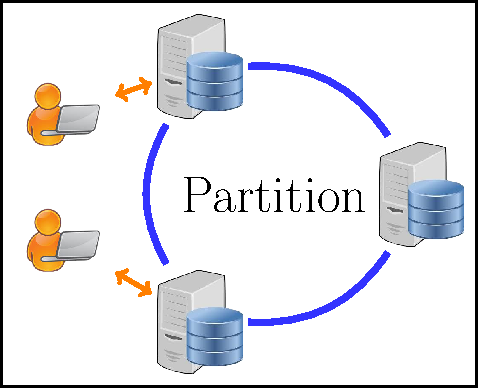
\includegraphics[scale = 0.80]{figs/partition.pdf}}; 
  }
  \uncover<3->{
    \node (partition-right) [] at (6, 3.5) {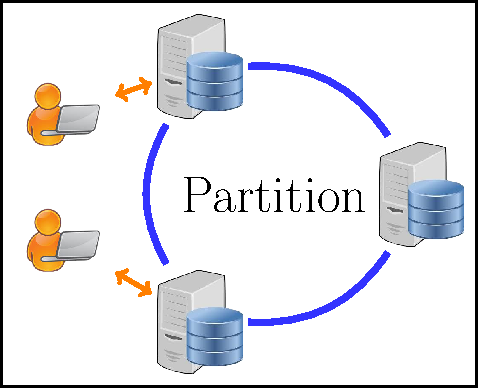
\includegraphics[scale = 0.80]{figs/partition.pdf}}; 
    \node (partition-below) [] at (1.5, -5) {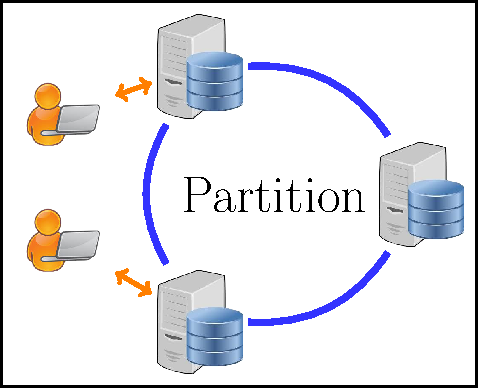
\includegraphics[scale = 0.80]{figs/partition.pdf}}; 

    % connections among partitions
    \draw [connection] (partition-left) to (partition-right); 
    \draw [connection] (partition-right) to (partition-below);
    \draw [connection] (partition-below) to (partition-left);

    % replication 
    \node (replication) [font = \Huge, align = center] at (0.5, 0.0) {\textbf{Wide-area}\\[3pt]\textbf{Replication}};
  }

  \uncover<4->{
    % master-slave for one partition
    \begin{scope}[circled/.style = {draw, circle, dash pattern = on 10pt off 5pt, cyan, line width = 2pt, outer sep = 5pt, minimum size = 2.0cm}, 
      conn/.style = {dash pattern = on 15pt off 8pt, cyan, line width = 2pt}]
    \node (ms-left) [circled] at (-4., 1) {};
    \node (ms-right) [circled] at (5.5, 1.7) {};
    \node (ms-below) [circled] at (4., -5.0) {};

    \node (master-slave) [below right = 1.5cm and -1.5cm of partition-right] {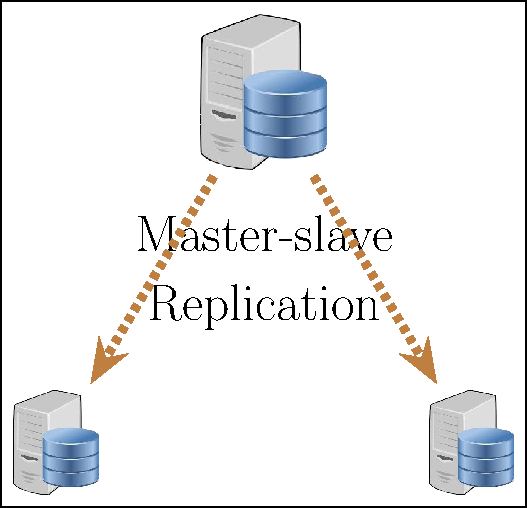
\includegraphics[scale = 0.80]{figs/master-slave.pdf}};
    \draw [conn] (ms-left) to (master-slave);
    \draw [conn] (ms-right) to (master-slave);
    \draw [conn] (ms-below) to (master-slave);
    \end{scope}
  }
\end{tikzpicture}
}
  \end{center}

  \begin{center}
    \only<2>{Keys are \textbf{partitioned} within a single datacenter.}
    \only<3-4>{Each key is \textbf{replicated} across datacenters} \only<4>{in a \textbf{master-slave} manner.}
    \only<5>{Transactions are first executed and committed on the \textbf{masters},\\
      and are then asynchronously propagated to \textbf{slaves}.}
  \end{center}
\end{frame}
%%%%%%%%%%%%%%%

%%%%%%%%%%%%%%%
\begin{frame}{}
  \begin{center}
    \only<1,3->{\resizebox{0.60\textwidth}{!}{\begin{tikzpicture}[]
% client library: transactional api + rvsi api + context api
\begin{scope}[clib/.style = {draw, rectangle, rounded corners, font = \LARGE, inner sep = 8pt, minimum width = 4cm}]
  \node (tx-api) [clib, outer sep = 5pt] at (0,0) {Transactional API};
  \node (rvsi-api) [clib, right = of tx-api] {RVSI API};
  \node (ctx-api) [clib, left = of tx-api] {Context API};

  % client library text
  \node (client-library-text) [font = \huge, above = 0.40cm of tx-api, blue] {Client Library};

  % surrounding
  \begin{pgfonlayer}{background}
    \node (client-library-surrounding) [blue, ultra thick, rectangle, draw, inner sep = 5pt, fit = (tx-api) 
    (rvsi-api) (ctx-api) (client-library-text)] {};
  \end{pgfonlayer}
\end{scope}

% distributed transaction:
\begin{scope}[master/.style = {rectangle, rounded corners, font = \huge, inner sep = 8pt}, 
	dist-tx/.style = {>=Stealth, <->, outer sep = 3pt, thick}]
  % two masters
  \node (master-left) [master, below left = 3.0cm and 1.0cm of tx-api.south] {Master};
  \node (master-right) [master, below right = 3.0cm and 1.0cm of tx-api.south] {Master};
  \draw [>=Stealth, <->, bend right = 45, thick] (master-left) to node[font = \LARGE, sloped, below] {Partition} (master-right);

  % master surrounding
  \begin{pgfonlayer}{background}
    \node (master-surrounding) [rectangle, rounded corners, draw, inner sep = 8pt, outer sep = 5pt,
		fit = (master-left) (master-right)] {};
  \end{pgfonlayer}

  % distributed transaction
  \draw [dist-tx] (tx-api) to (master-surrounding.155);
  \draw [dist-tx] (tx-api) to (master-surrounding.25);
  \node (dist-tx-text) [font = \LARGE, above = 1.00cm of master-surrounding.north, align = center, red] {RVSI-MP};
\end{scope}

% replication
\begin{scope}[slave/.style = {rectangle, rounded corners, font = \LARGE, inner sep = 8pt}, 
  	rep/.style = {>=Stealth, ->, draw, thick}]
  % slaves of master-left
  \node (slave-left-above) [slave, below left = 1.0cm and 2.2cm of master-left] {Slave};
  \node (slave-left-below) [slave, below right = 2.5cm and 0.20cm of slave-left-above] {Slave};
  \draw [rep] (master-left) to (slave-left-above);
  \draw [rep] (master-left) to node[sloped, font = \LARGE, above] {Replication} 
  node[sloped, font = \LARGE, below = 5pt, red] {RVSI-MS} (slave-left-below);
  % slaves of master-right
  \node (slave-right-above) [slave, below right = 1.0cm and 2.2cm of master-right] {Slave};
  \node (slave-right-below) [slave, below left = 2.5cm and 0.20cm of slave-right-above] {Slave};
  \draw [rep] (master-right) to (slave-right-above);
  \draw [rep] (master-right) to node[sloped, font = \LARGE, above] {Replication} 
  node[sloped, font = \LARGE, below = 5pt, red] {RVSI-MS} (slave-right-below);
\end{scope}


% data store surrounding
\begin{pgfonlayer}{background}
  \node (datastore-surrounding) [draw, rectangle, inner sep = 10pt, 
	fit = (master-left) (master-right) (slave-left-above) (slave-left-below) (slave-right-above) 
	  (slave-right-below) (master-surrounding)] {};
\end{pgfonlayer}

% data store text
\node (datastore-text) [above = 0.20cm of datastore-surrounding.south, font = \huge] {Key-value Store};

% client
\begin{scope}[access/.style = {>=Stealth, <->, thick}]
  \node (client) [above = 2.0cm of client-library-surrounding, draw, font = \huge, rectangle, inner sep = 10pt, minimum width = 15.0cm] {Clients};
  \coordinate (client-left) at ($ (client.south west) ! 0.20 ! (client.south east)$);
  \coordinate (client-right) at ($ (client.south west) ! 0.80 ! (client.south east)$);
  \draw [access] (client-left) to node [left, font = \Large, align = center] 
	{\textsc{Begin}\\\textsc{End}} (client-left |- client-library-surrounding.north);
  \draw [access] (client-right) to node [right, font = \Large, align = center] 
	{\textsc{read}\\\textsc{write}}(client-right |- client-library-surrounding.north);
\end{scope}

% rvsi-ms
\only<4>{
\begin{scope}
  \node () [draw, rectangle, rounded corners, rotate fit = 45, very thick, teal, 
  fit = (master-left) (slave-left-above) (slave-left-below)] {};
\end{scope}
}

% rvsi-mp
\only<5>{
\begin{scope}
  \node () [draw, rectangle, rounded corners, very thick, teal, 
  fit = (master-left) (master-right) (dist-tx-text)] {};
\end{scope}
}
\end{tikzpicture}}}
  \end{center}

  \begin{center}
    \only<1>{\blue{Client library}}
    \only<3>{\red{\rvsi{} protocol: \rvsims{} + \rvsimp{}}}
    \only<4>{\textcolor{teal}{\rvsims{}}: \rvsi{} for Master-Slave replication}
    \only<5>{\textcolor{teal}{\rvsimp{}}: \rvsi{} for Multiple Partitions}
  \end{center}

  \only<2>{
    \centerline{Code snippet for writing \rvsi{} transactions:}
    \vspace{0.30cm}
    \begin{lstlisting}[
  language = Java,
  basicstyle = \ttfamily\footnotesize,
  showstringspaces = false,
  keywordstyle = \color{blue}\bfseries,
  commentstyle = \color{teal},
  stringstyle = \bfseries,
  upquote = true,
  frame = box,
  breaklines = true,
  linewidth = 0.85\textwidth
]
  // Initialize keys (ck, ck1, and ck2) here
  ITx tx = new RVSITx(/** context **/);

  tx.begin();

  // Read and write
  ITsCell tsCell = tx.read(ck);
  ITsCell tsCell1 = tx.read(ck1);
  tx.write(ck1, new Cell("R1C1"));
  ITsCell tsCell2 = tx.read(ck2);

  // Specify RVSI specs. (e.g., SVSpec)
  RVSISpec sv = new SVSpec();
  sv.addSpec({ck, ck1, ck2}, 2);
  tx.collectRVSISpec(sv);

  boolean committed = tx.end();
\end{lstlisting}

  }
\end{frame}
%%%%%%%%%%%%%%%
